\documentclass[12pt,fleqn]{article}
\setlength{\parindent}{0pt}
\usepackage{graphicx}
\usepackage{listings}
\usepackage[latin5]{inputenc}
\setlength{\parskip}{8pt}
\setlength{\parsep}{0pt}
\setlength{\headsep}{0pt}
\setlength{\topskip}{0pt}
\setlength{\topmargin}{0pt}
\setlength{\topsep}{0pt}
\setlength{\partopsep}{0pt}
\setlength{\mathindent}{0cm}

\begin{document}
MIT OCW Cok Degiskenli Calculus - Ders 2

Onceki derste iki uygulama gorduk. Ucuncu bir uygulama bir $\vec{A}$
vektorunun bir birim vektor $\vec{u}$ yonundeki bilesenlerini /
parcalarinin (components) hesaplanmasidir.

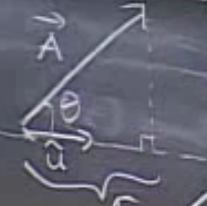
\includegraphics[height=3cm]{2_1.png}

Ustteki sekilde $\vec{A}$'nin $\vec{u}$ yonundeki ``yansimasini'' goruyoruz
ve bu yansima $\vec{A}$'nin $\vec{u}$ yonundeki bilesenidir,
buyuklugudur. 

Aradaki a�� $\theta$ ise ve ucgen dik ise, o zaman bu yansima 

\[ |\vec{A}| cos(\theta) \]

olarak hesaplanacaktir. Bu formulun ilk hali aslinda

\[ |\vec{A}| |\vec{u}| cos (\theta) \]

fakat $\vec{u}$ birim vektor olduguna gore, uzunlugu 1, o zaman bu buyukluk
carpimdan atilabilir.  Ustteki formul ayni zamanda bir noktasal carpim,
$\vec{A}\cdot\vec{u}$.

Eger bir vektorun mesela $\hat{i}$ yonundeki yansimasini almak isteseydik,

\[ \vec{A} \cdot \hat{i} \]

kullanirdik, bu da

\[ \vec{A} \cdot <1,0,0>\]

olurdu. Bu carpim $x$ yonunde 1 ile carpar diger tum eksenleri sifirlar,
yani diger bir degisle $\vec{A}$'nin $x$ yonundeki bilesenini hesaplamis oluruz. Bu
arada $\hat{i}$ tabii ki bir birim vektor. Uzunlugu 1.

Uygulama 

Fizikte, yuvarlak bir sekilde donebilen bir sarkac problemini dusunelim. Bu
sistemi analiz etmek icin Newton Kanunu, mekanik, vs. kullanmaniz gerekir
tabii ki, fakat vektorler  geometrik olarak bu sistemi anlamak icin cok
faydalidir. 

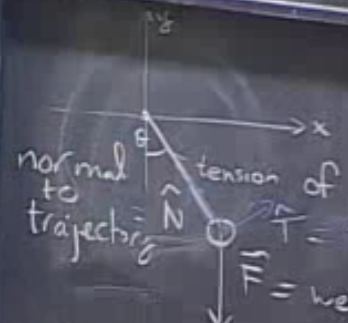
\includegraphics[height=4cm]{2_2.png}

Bu sarkacin ileri geri sallanmasinin sebebi ustte takip edilen yuvarlak
yoldur. Analiz icin $x, y$ yonundeki bilesenlere bakmak yerine belki de
resimdeki iki birim vektor yonune bakmamiz lazim, ki bu vektorlerden biri
takip edilen yola teget yonu gosteren $\vec{T}$, digeri yuvarlak tanjantina
dik olan $\vec{N}$. O zaman agirligi temsil eden $\vec{F}$'in bu iki vektor
yonundeki bilesenlerine bakabiliriz.

Resimde ipin gerginligi (tension of string) $\vec{N}$ yonunde, bu yon ip
gerginligi yonu, $\vec{F}$'in $\vec{N}$ yonundeki bileseni gerginligi
yaratan faktordur. $\vec{F}$'in tegetlik yani $\vec{T}$ yonundeki bileseni ise
ileri geri hareketi saglayan faktordur.

Muhakkak sarkacin $y$ ekseni ile olusturdugu bir a�� $\theta$ uzerinden bir
suru cos, sin terimleri iceren denklemler ortaya cikartabilirdiniz, bu
ilginc olurdu, fakat eger daha kisa bir yolu takip etmek istiyorsak,
noktasal carpim kullaniriz. 

Vektorler baglaminda anlamamiz gereken bir diger kavram, alan
kavrami. Diyelim ki elimizde bir pentagon sekli var. Bu seklin alanini
vektorler kullanarak hesaplayabilir miydik? 

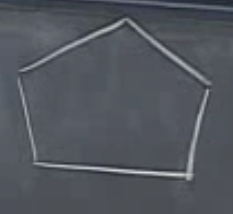
\includegraphics[height=2cm]{2_3.png}

Evet hesaplayabiliriz. Problemi basitlestirelim. Pentagonu ucgenlere
ayiralim. 

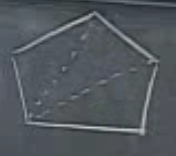
\includegraphics[height=2cm]{2_4.png}

sonra bu alanlari toplayalim. Ucgen alanini nasil hesaplariz? Soyle bir
ucgen dusunelim

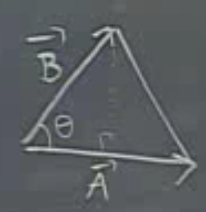
\includegraphics[height=2cm]{2_5.png}

Bu ucgenin alani

\[ \frac{1}{2}|\vec{A}||\vec{B}|sin(\theta) \]

Bu formul $cos$ iceren diger formulumuze benziyor. Bundan istifade
edebiliriz belki. Once $cos(\theta)$'yi buluruz, sonra $sin^2\theta + cos^2\theta
= 1$ esitligini 
kullanarak $sin(\theta)$'yi buluruz.

Fakat bu gereginden fazla is yaratir. Daha kolay bir yontem var. Bu yontem
icin determinantlar kullanmak lazim. 

Devam edelim: Madem a��larin cos degerlerini bulmayi biliyoruz, belki oyle
bir diger a�� bulmaliyiz ki o a��nin cos degeri bizim aradigimiz a��nin sin
degeri olsun, cunku alan icin sin gerekiyor, ama hesaplayabildigimiz cos. 

Birbirini tamamlayici a��lar (complemantary angles) kavramini biliyoruz
herhalde. 

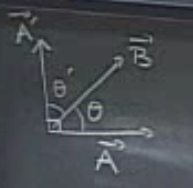
\includegraphics[height=3cm]{2_6.png}

Diyelim ki elimizde $\vec{A}$ var, onu $90^o$ cevirip ustteki hale getiriyoruz,
yeni vektore $\vec{A'}$ diyelim. O vektor ile $\vec{B}$ arasindaki a��ya da
$\theta'$ diyelim. 

\[ \theta' = \frac{\pi}{2} - \theta \]

\[ cos(\theta') = sin(\theta) \]

Bu demektir ki 

\[ |\vec{A}||\vec{B}|sin\theta = |\vec{A'}||\vec{B}|cos\theta'  \]

$|\vec{A}|$ yerine $|\vec{A'}|$ koymakla hicbir sey degistirmiyorum cunku
bu vektorlerin yonleri degisik olsa da buyuklukleri ayni. Devam edelim,
ustteki formulde sag tarafi basitlestirirsek

\[ = \vec{A'} \cdot \vec{B} \]

Bu temiz bir formul. Tek eksik, $\vec{A'}$'nin ne oldugunu hala
hesaplamadik. Fakat bunu yapmak o kadar zor degil. Bunun icin $\vec{A}$'yi
cevirebilmemiz lazim. Alttaki resme bakalim, 

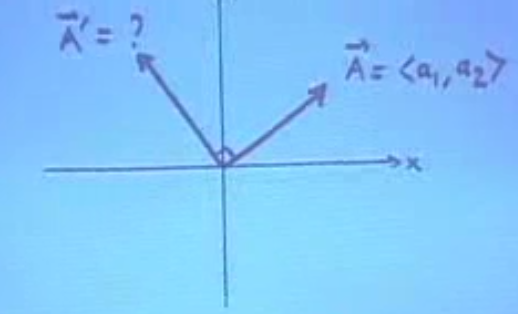
\includegraphics[height=4cm]{2_7.png}

acaba $\vec{A'}$ ne olur?  Secenekler [bu hoca boyle ufak sinavlari
seviyor, faydali aslinda, bu sinavlara gelince siz de cevabini vermeye
ugrasin].

\begin{enumerate}
   \item $<a_2,a_1>$
   \item $<a_2,-a_1>$
   \item $<-a_2,a_1>$
   \item $<-a_1,a_2>$
   \item Hicbiri
\end{enumerate}

Dogru cevap: 3. 

Bu nasil oldu? Alttaki resme bakalim

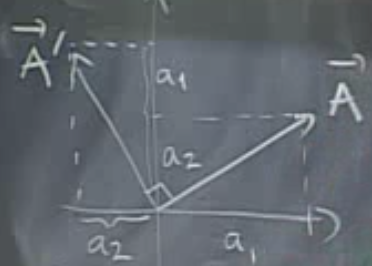
\includegraphics[height=4cm]{2_8.png}

$\vec{A}$'nin etrafinda bir dikdortgen hayal edelim, ve dikdortgeni
icindeki vektor ile beraber alip sola dogru ceviriyoruz. O zaman uzun kenar
artik yukari dogru bakiyor, yani $a_1$ yukari bakiyor, $a_2$ nin de yeri
degisiyor, yani bu buyuklukler yer degistiriyorlar. Ayrica $a_2$ artik ters
yone gittigi icin isareti degisiyor.

O zaman su formule donersek

\[ = \vec{A'} \cdot \vec{B} \]

soyle olur

\[ a_1b_2 - a_2b_1 \]

Bu formul determinantlardan tanidik gelebilecek bir formul, 

\[ = det(\vec{A},\vec{B}) \]

Aslinda $\vec{A},\vec{B}$ ile bu vektorleri yanyana kolonlara koydugumuz su
formu dusunuyoruz ve onun determinantini aliyoruz

\[ =
\left|\begin{array}{rr}
a_1 & a_2 \\
b_1 & b_2 \\
\end{array}\right|
 \]

Ve bu determinant hesabinin sonucu kenarlari $\vec{A}$ ve $\vec{B}$ olan
bir paralelogramin alanidir. Tabii paralelogram icindeki ucgeni istiyorsak
bu sonucu ikiye boleriz. 

Not: Alan pozitif bir seydir, fakat $a_1b_2 - a_2b_1$'in kesinlikle pozitif
cikmasinin garantisi yoktur. Eksi degerli terimler buyuyup arti degerlileri
asabilirler. O zaman ifadelerimizin tam dogru olmasi icin ustteki
determinant hesabi -alan ya da +alan degerine esittir demek lazim. 



\end{document}
